%Writeup for ENGR202 Lab 6 
%If editing in vim/vi please insert your own line breaks! This will help keep the file cleaner and easier to edit.

%::Collaboration etiquette::
%In order to better identify changes
%please surround all edits with your
%name as follows:

%BEGIN Zach
%END Zach

%LaTeX will ignore line breaks so to denote
%changes in the middle of a line begin the
%edits on a new line after your name tag
%and then continue with the original on
%the next line following your ending name
%tag.



\documentclass{article}
\usepackage{graphicx}
\graphicspath{ {images/} }

%Change # to correct lab number!
\title{Chapter #6 Lab Writeup}
\author{Zach Thompson, Simon Hannes, Kyle Peterson}
\begin{document}

\maketitle{}

%BEGIN SIMON
\section*{Introduction}
The goal of this Lab is to put together all the information we've amassed 
during the last 9 weeks of class in building a filter network with three
distinct filters catered to specific types of speakers. These filters will
be:
\begin{enumerate}
\item a low pass filter designed for use with a subwoofer
\item a bandpass filter designed for use with the speaker provided in our lab kits
\item a high pass filter designed for use with a tweeter
\end{enumerate}

We then will connect this filter network to appropriate amplification for each 
filter, and out to the speakers. In addition, we will make the system mobile
 and add in a potentiometer to vary the volume, plus an LED to show when the 
network is receiving power.

\section*{Design}
The capacitors available for use were $0.1\mu F$, $1\mu F$ and $10\mu F$. We 
were warned against using resistor values of less than $100\Omega$.

The first consideration we made was determining the frequency range which 
we hoped to encompass by each filter. We used cutoff frequencies of 200Hz
for the low pass, 6kHz for the high pass, and 500Hz, 5kHz for the band-pass.
We used the equation: $Fcutoff = 1/(2\pi*RC)$ to determine capacitor and 
resistor values for each filter. Our initial guesses were shown to be fairly 
functional when modeled in LTSpice, with the exception of the band-pass which 
needed slight modification to achieve an amplitude which matched the amplitude 
created by the other two  filters. To do this, we increased the resistance
in the high-pass section of  the band-pass, and lowered the attached capacitor
by a factor of ten. The values are as follows:
\begin{enumerate}
\item LOW-PASS: $200Hz=795\mu$ seconds. We chose a $1\mu$ capacitor and 
$795\Omega$ worth of resistors.
\item HIGH-PASS: $6kHz=27\mu$ seconds. We chose a $0.1\mu$ capacitor and 
$270\Omega$ worth of resistors. 
\item BAND-PASS: For the low-end, we found $400Hz=40\mu$ seconds. We chose a 
$0.1\mu$ capacitor and $400\Omega$ worth of resistors. For the high-end, we found
$2kHz=20\mu$ seconds. For this we chose a $0.1\mu$ capacitor and $2000\Omega$
worth of resistors.
\end{enumerate}
%END SIMON

\section*{Simulations and Testing}
<<<<<<< HEAD

%BEGIN SIMON
=======
%BEGIN KYLE
\begin{figure}[!h]
\centering
\caption{Schematic}
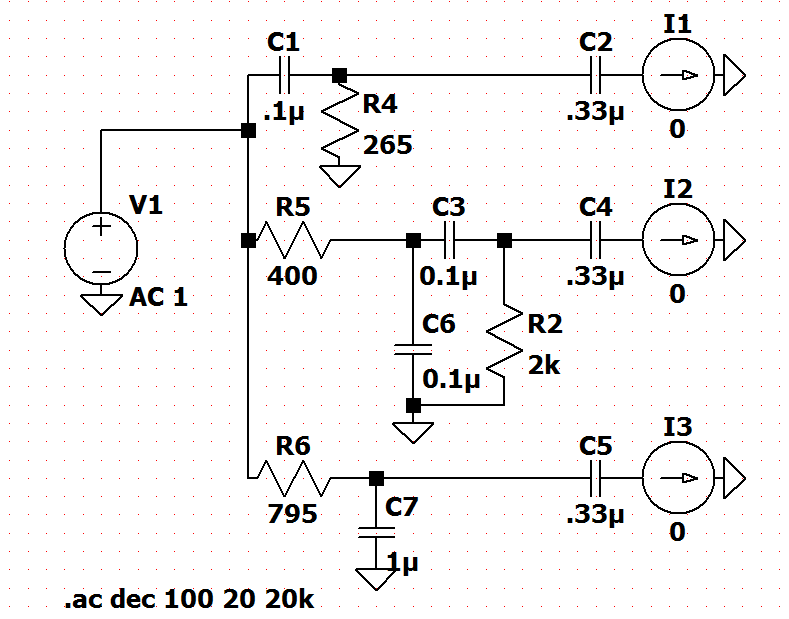
\includegraphics[scale=.5]{lab6_spice_schematic}
\caption{Simulation Results}
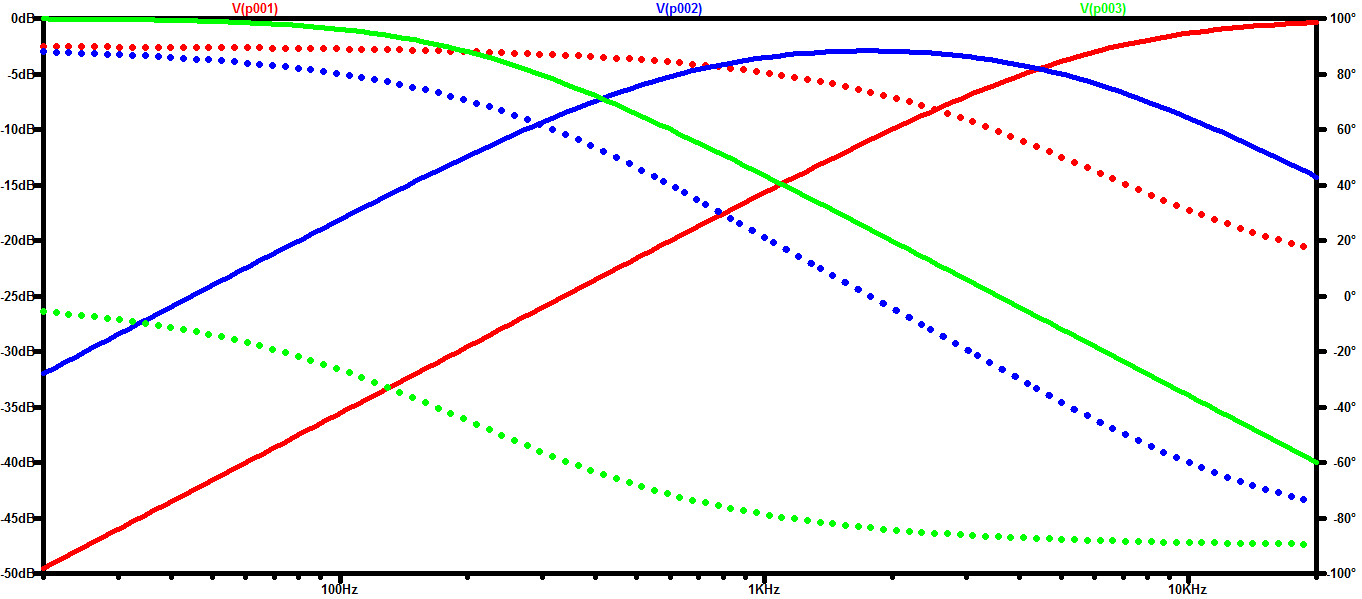
\includegraphics[width=\linewidth]{lab6_spice_graph}
\end{figure}

\begin{figure}[!ht]
\caption{Data Table}
\begin{center}
\begin{tabular}{|c|c|c|c|c|}
\hline
Freq (Hz)&Vin(V)&High(mV)&Mid(mV)&Low(mV)\\
\hline
10&5&14.4&72&2000\\
\hline
30&5&28&196&2000\\
\hline
100&5&92&664&2000\\
\hline
300&5&200&1380&2000\\
\hline
1000&5&600&2000&849\\
\hline
3000&5&1120&1720&150\\
\hline
10000&5&1560&640&86\\
\hline
30000&5&1560&240&50\\
\hline
\end{tabular}
\begin{flushleft}
We had trouble with the osciloscope clipping at 2V, so we do not have data above 2V. To help combat this issue the function generator was set to 256mV rather than 1V.
\end{flushleft}
\end{center}
\end{figure}
\begin{figure}[!h]
\centering
\caption{Magnitude Vs Frequency}
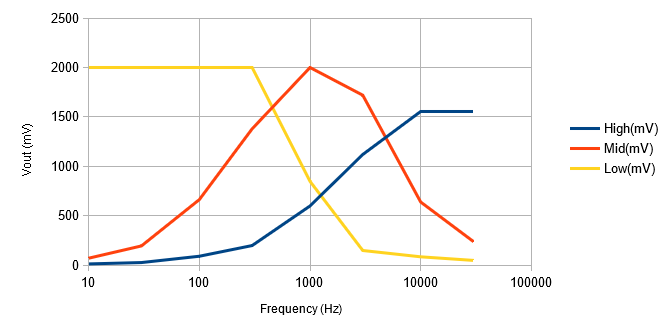
\includegraphics[width=\linewidth]{magnitudevsfrequency}
\end{figure}
%END KYLE
>>>>>>> 702e19e874745e2248b3bd0f3907afd7ee5d0a77
\section*{Results}
We succeeded in creating a 3 stage filter network which plays music out of 
three different speakers. Huzzah! It was satisfying to see the final result
of our effort. In conclusion, we found great success in this project, from design, 
to consruction, to testing. We found results which matched our expectations 
from design. 

Thankfully, all the issues we encountered were overcome with a bit of effort. 
After constructing the filter network, we attempted to power it using the 
power supply that Simon had constructed in ECE 112, resulting in a very noisy 
signal. We added an inductor inline before the board and the noise was 
neutralized. We noticed the amps were running very hot, so we added a fan and 
some heat sync glue to draw off excess heat. 


\section*{Conclusion}
We began by setting cutoff values from speaker output values. We used these 
cutoff values to determine resistor and capcitor values. We then had 
everything we needed to construct the circuit. We made a mock-up on a 
breadboard to test that our design worked, which it did. We then handed 
over the reins to our master solder-tech, Zach, who did a marvellous 
job of connecting the components in a compact and organized way. With 
the final product fully cocnstructed, we just some final testing to 
make sure that everything worked as expected. If we were able to do this 
project again, there isn't much we would change. 

\section*{Extra Credit}
We added in several extra components to increase the functionality of the 
device including:
\begin{enumerate}
\item An LED to show when the device is powered
\item A fan to deal with heat created by the amps which were found to be in
 excess of 110 degrees.
\item An on and off switch for the signal. 
\item A potentiometer installed before the filters in the signal path to 
control volume.
\item Powered the circuit via a 5V battery pack.
\end{enumerate}
%END SIMON
\end{document}
